
\documentclass[a4paper,11pt]{article}
\usepackage{amsmath,amsthm,amsfonts,amssymb,amscd,amstext,vmargin,graphics,graphicx,tabularx,multicol} \usepackage[french]{babel}
\usepackage[utf8]{inputenc}  
\usepackage[T1]{fontenc} 
\usepackage[T1]{fontenc}
\usepackage{amsmath,amssymb}
\usepackage{pstricks-add,tikz,tkz-tab,variations}
\usepackage[autolanguage,np]{numprint} 
\usepackage{color}
\usepackage{ulem}

\setmarginsrb{1.5cm}{0.5cm}{1cm}{0.5cm}{0cm}{0cm}{0cm}{0cm} %Gauche, haut, droite, haut
\newcounter{numexo}
\newcommand{\exo}[1]{\stepcounter{numexo}\noindent{\bf Exercice~\thenumexo} : \marginpar{\hfill /#1}}
\reversemarginpar


\newcounter{enumtabi}
\newcounter{enumtaba}
\newcommand{\q}{\stepcounter{enumtabi} \theenumtabi.  }
\newcommand{\qa}{\stepcounter{enumtaba} (\alph{enumtaba}) }
\newcommand{\initq}{\setcounter{enumtabi}{0}}
\newcommand{\initqa}{\setcounter{enumtaba}{0}}

\newcommand{\be}{\begin{enumerate}}
\newcommand{\ee}{\end{enumerate}}
\newcommand{\bi}{\begin{itemize}}
\newcommand{\ei}{\end{itemize}}
\newcommand{\bp}{\begin{pspicture*}}
\newcommand{\ep}{\end{pspicture*}}
\newcommand{\bt}{\begin{tabular}}
\newcommand{\et}{\end{tabular}}
\renewcommand{\tabularxcolumn}[1]{>{\centering}m{#1}} %(colonne m{} centrée, au lieu de p par défault) 
\newcommand{\tnl}{\tabularnewline}

\newcommand{\trait}{\noindent \rule{\linewidth}{0.2mm}}
\newcommand{\hs}[1]{\hspace{#1}}
\newcommand{\vs}[1]{\vspace{#1}}

\newcommand{\N}{\mathbb{N}}
\newcommand{\Z}{\mathbb{Z}}
\newcommand{\R}{\mathbb{R}}
\newcommand{\C}{\mathbb{C}}
\newcommand{\Dcal}{\mathcal{D}}
\newcommand{\Ccal}{\mathcal{C}}
\newcommand{\mc}{\mathcal}

\newcommand{\vect}[1]{\overrightarrow{#1}}
\newcommand{\ds}{\displaystyle}
\newcommand{\eq}{\quad \Leftrightarrow \quad}
\newcommand{\vecti}{\vec{\imath}}
\newcommand{\vectj}{\vec{\jmath}}
\newcommand{\Oij}{(O;\vec{\imath}, \vec{\jmath})}
\newcommand{\OIJ}{(O;I,J)}

\newcommand{\bmul}[1]{\begin{multicols}{#1}}
\newcommand{\emul}{\end{multicols}}


\newcommand{\reponse}[1][1]{%
\multido{}{#1}{\makebox[\linewidth]{\rule[0pt]{0pt}{20pt}\dotfill}
}}

\newcommand{\titre}[5] 
% #1: titre #2: haut gauche #3: bas gauche #4: haut droite #5: bas droite
{
\noindent #2 \hfill #4 \\
#3 \hfill #5

\vspace{-1.6cm}

\begin{center}\rule{6cm}{0.5mm}\end{center}
\vspace{0.2cm}
\begin{center}{\large{\textbf{#1}}}\end{center}
\begin{center}\rule{6cm}{0.5mm}\end{center}
}



\begin{document}
\pagestyle{empty}
\titre{Devoir type Brevet}{Nom :}{Prénom :}{3 ème}{Date :}


\exo{4,5} 

\q Calculer les expressions $A$ et $B$. On écrira les résultats sous la forme de fractions aussi simples que possible.

\bmul{2}

$A = \dfrac{3}{8} - \dfrac{7}{8} \times \dfrac{4}{3}$

\columnbreak

$B = (\dfrac{1}{3} - \dfrac{1}{4}) \div \dfrac{2}{3} +1$
\emul

\q Donner l'écriture scientifique de $D$ en précisant les
différentes étapes de calcul.

\begin{center}
$D = \dfrac{6 \times 10^{-1} \times 7 \times 10^{4}}{12 \times (10^{3})^{3}}$\\
\end{center}

\exo{4 } Soit l'expression $E= (5x-3)^{2} - (4x + 1)^{2}$\\

\noindent \initq \q Développer et réduire l'expression $E$.\\
\q Factoriser l'expression $E$.\\
\q Calculer l'expression $E$ pour $x= 0$ et $x=-1$.\\


\exo{4} On considère un rectangle $ABCD$ tel que $AB=8$~cm et $BC=5$~cm. Sur le segment $[CD]$, on place le point $M$ tel que $CM=6$~cm.\\

\noindent \initq \q Calculer la mesure de l'angle $\widehat{MBC}$, arrondie au degré près.\\
\q On note $N$ le point d'intersection des droites $(BM)$ et
$(AD)$. Représenter la figure en grandeur réelle.\\
\q Calculer les longueurs $BM$ et $DN$, arrondies au millimètre près.\\



\exo{5}

\bmul{2}

\includegraphics[scale=1]{dmbrevet1.eps}  

\columnbreak

On donne les informations suivantes pour la figure ci-contre  :\\


\noindent - (AC) est parallèle à (EF)\\
- AB = 5,8 cm ;\\
– BC = 9,4 cm ;\\
– BF = 3 cm ;\\
– EB = 3 cm ;\\
– EF = 3,5 cm.\\


\noindent \initq \q Calculer la longueur BD, arrondie au millimètre près.\\
\q Calculer AD : donne la valeur exacte puis la
valeur arrondie au dixième.\\
\q Calculer la longueur AC, arrondie au millimètre près. En déduire DC.

\emul


\exo{3,5} \\


\includegraphics[scale=1]{dmbrevet1bis.eps} \\

\initq \q Pour  réaliser  la  figure  ci-dessus, on a défini un motif en forme de losange et on a utilisé l'un des deux 
programmes A et B ci-dessous.\\
Déterminer  lequel  et  indiquer  par  une  figure  à  main  levée  le  résultat  que  l'on  obtiendrait  avec  l'autre 
programme.\\

\begin{flushleft}
 \includegraphics[scale=0.9]{dmbrevet1ter.eps}
 \end{flushleft} 



\q Combien mesure l'espace entre deux motifs successifs ?\\

\q On souhaite réaliser la figure ci-dessous :\\


\includegraphics[scale=1]{dmbrevet1qua.eps} 


Pour ce faire, on envisage d'insérer l'instruction 
\includegraphics[scale=0.8]{dmbrevet1cinq.eps}  dans le programme utilisé à la question 1. \\
Où faut-il insérer cette instruction ?\\


\end{document}
